\section{Vai trò của các thành phần trong hệ thống}

Mỗi thành phần trong hệ thống đảm nhiệm một vai trò riêng, đồng thời phối hợp với các thành phần khác để tạo thành một quy trình xử lý hoàn chỉnh. Việc phân chia rõ ràng vai trò giúp hệ thống dễ bảo trì, dễ mở rộng và phù hợp với mô hình triển khai thực tế.

\subsection{Frontend Web}

Frontend Web là lớp giao diện người dùng của hệ thống. Đây là nơi người dùng trực tiếp tương tác với trợ lý ảo thông qua trình duyệt web.

Các chức năng chính:
\begin{itemize}
    \item Hiển thị giao diện chat giữa người dùng và trợ lý ảo.
    \item Gửi câu hỏi của người dùng đến Backend API.
    \item Hiển thị câu trả lời từ Rasa hoặc RAG.
    \item Hiển thị thông tin tuyển sinh: ngành học, phương thức xét tuyển, học phí, chỉ tiêu.
    \item Hỗ trợ đăng nhập, đăng ký và quản lý thông tin người dùng.
    \item Hiển thị lịch sử hội thoại và nguồn trích dẫn khi có.
    \item Cung cấp giao diện quản trị cho cán bộ tuyển sinh hoặc quản trị viên.
\end{itemize}

\subsection{Backend API}

Backend API là lớp trung gian giữa Frontend, Rasa Server, cơ sở dữ liệu và các phân hệ xử lý khác.

Các nhiệm vụ chính:
\begin{itemize}
    \item Cung cấp API cho Frontend Web.
    \item Quản lý đăng ký, đăng nhập, xác thực và phân quyền người dùng.
    \item Lưu trữ và truy xuất dữ liệu từ cơ sở dữ liệu quan hệ.
    \item Gửi tin nhắn đến Rasa Server và nhận phản hồi trả về Frontend.
    \item Cung cấp API quản trị cập nhật dữ liệu tuyển sinh.
    \item Ghi log hội thoại, lịch sử truy vấn, phản hồi và kiểm soát lỗi.
\end{itemize}

\subsection{Rasa Server}

Rasa Server là thành phần xử lý hội thoại chính trong hệ thống. Rasa tiếp nhận tin nhắn từ Backend API, phân tích ngôn ngữ tự nhiên, xác định ý định và quyết định hành động tiếp theo.

Các chức năng:
\begin{itemize}
    \item Phân tích intent, trích xuất entity.
    \item Quản lý trạng thái hội thoại, rule, story và form.
    \item Trả lời trực tiếp bằng template cho câu hỏi đơn giản.
    \item Gọi Action Server khi cần xử lý nghiệp vụ hoặc truy vấn dữ liệu.
    \item Chuyển tiếp sang RAG khi câu hỏi vượt ngoài phạm vi intent đã huấn luyện.
\end{itemize}

\subsection{Action Server}

Action Server là thành phần mở rộng của Rasa để thực thi hành động tùy chỉnh.

Nhiệm vụ chính:
\begin{itemize}
    \item Nhận yêu cầu action từ Rasa.
    \item Gọi Backend API hoặc RAG tùy ngữ cảnh.
    \item Xử lý dữ liệu trả về, định dạng câu trả lời.
    \item Trả kết quả về Rasa để gửi lại người dùng.
\end{itemize}

\subsection{Phân hệ RAG}

Phân hệ RAG (Retrieval-Augmented Generation) hỗ trợ truy hồi tri thức từ tài liệu tuyển sinh và sinh câu trả lời có căn cứ.

Các nhiệm vụ chính:
\begin{itemize}
    \item Tiếp nhận và chuẩn hóa câu hỏi.
    \item Tìm kiếm ngữ nghĩa trong Vector Store.
    \item Truy xuất nội dung từ Document Store.
    \item Kết hợp quan hệ từ Knowledge Graph khi cần.
    \item Xếp hạng lại đoạn tài liệu, tạo prompt và gọi mô hình sinh.
    \item Trả câu trả lời kèm nguồn trích dẫn.
\end{itemize}

\subsection{Cơ sở dữ liệu quan hệ}

Cơ sở dữ liệu quan hệ lưu trữ dữ liệu có cấu trúc của hệ thống như người dùng, ngành học, chỉ tiêu, phương thức xét tuyển, điểm chuẩn, học phí, lịch sử hội thoại và log nghiệp vụ.

\subsection{Vector Store}

Vector Store lưu embedding của các đoạn tài liệu để thực hiện tìm kiếm ngữ nghĩa, giúp truy vấn hiệu quả ngay cả khi câu hỏi diễn đạt khác từ khóa trong tài liệu.

\subsection{Document Store}

Document Store lưu tài liệu gốc (PDF, DOCX, HTML, Markdown), văn bản đã trích xuất, các đoạn chia nhỏ và metadata. Thành phần này cung cấp nội dung gốc để trích dẫn trong câu trả lời.

\subsection{Knowledge Graph}

Knowledge Graph biểu diễn tri thức dạng thực thể -- quan hệ, ví dụ: ngành học thuộc khoa, ngành học dùng tổ hợp xét tuyển nào, phương thức nào áp dụng cho ngành nào. Thành phần này hữu ích cho câu hỏi quan hệ nhiều bước.

\subsection{Phân hệ quản trị}

Phân hệ quản trị phục vụ quản trị viên/cán bộ tuyển sinh trong các nghiệp vụ:
\begin{itemize}
    \item Quản lý tài khoản, vai trò, quyền hạn.
    \item Quản lý dữ liệu tuyển sinh, ngành học, tổ hợp, học phí, chỉ tiêu.
    \item Quản lý tài liệu, kích hoạt indexing và theo dõi đồng bộ Vector Store.
    \item Theo dõi lịch sử hội thoại, câu hỏi chưa trả lời được, log lỗi và hiệu năng.
\end{itemize}

\begin{figure}[H]
    \centering
    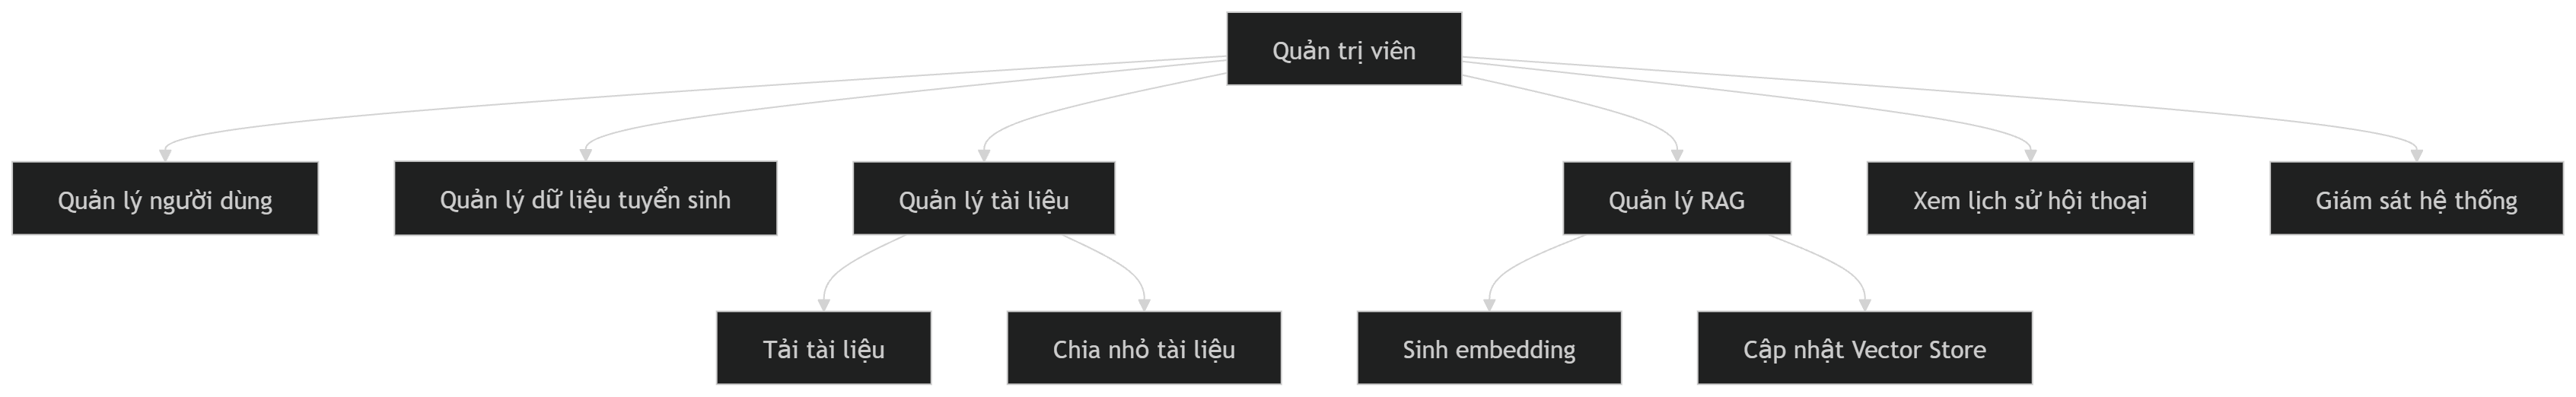
\includegraphics[width=0.95\textwidth]{content/source/Hình 3.2 Sơ đồ chức năng phân hệ quản trị..png}
    \caption{Sơ đồ chức năng phân hệ quản trị}
    \label{fig:admin_subsystem_functional_diagram}
\end{figure}
